% One source thumbnail and two reading paths per teaching page.
\clearpage
\begingroup
\newcounter{courseslide}
\newenvironment{slidenotes}[3]{%
  \ifnum#1=1\relax
    \section{Slide-by-slide syllabus companion}\label{app:slides}
    {\small Read either path, then compare explanations. Thumbnails reproduce the supplied slides unchanged; the notes clarify their interpretation. Slide numbers follow the presentation.}\par
  \else\clearpage\fi
  \begin{center}#3\end{center}\vspace{-2mm}
  \refstepcounter{courseslide}
  \subsection*{Slide #1. #2}\label{app:slide-#1}
  \addcontentsline{toc}{subsection}{Slide #1. #2}
  \small
}{\par}
\newcommand{\biopath}{\par\smallskip\textbf{Biomedical and imaging path}\par\nobreak}
\newcommand{\comppath}{\par\medskip\textbf{Computational path}\par\nobreak}

\begin{slidenotes}{01}{From brains to models}{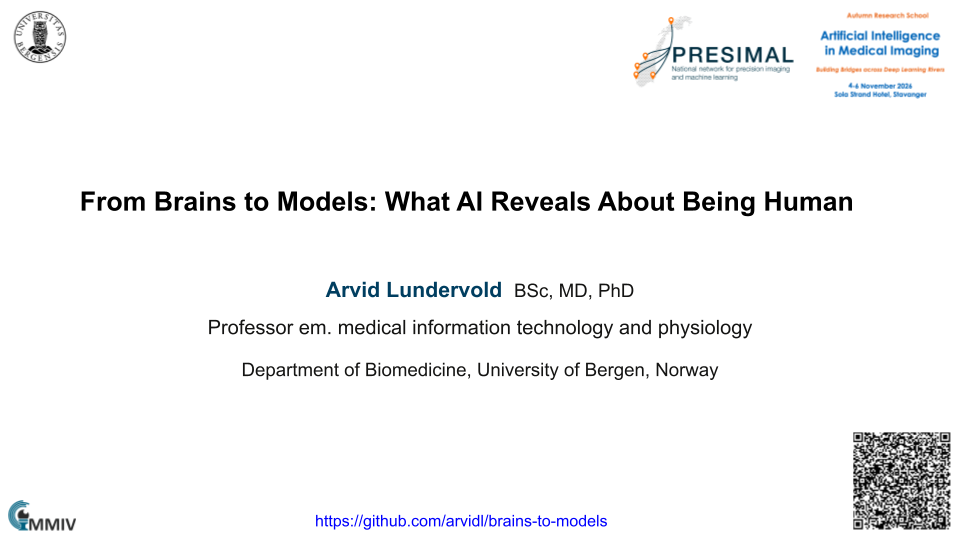
\includegraphics[width=.64\linewidth]{figures/talk/slide-01.png}}
\biopath
The title introduces a comparison between biological cognition and engineered systems. In medicine, the comparison becomes concrete when a model reads an image, produces a lesion outline, or drafts an explanation. Each activity resembles something a professional does, but resemblance leaves several questions open. Does the system detect the relevant tissue? Does it use the same evidence as the professional? Does its output help a patient? A successful answer to one question supplies a starting point for the next investigation.

Use three distinctions throughout this syllabus: performance, mechanism and consequence. Performance concerns what a system achieves under a specified test. Mechanism concerns how it achieves that result. Consequence concerns what happens when people act on it. For example, a more reproducible tumour-volume estimate could improve measurement without yet establishing a treatment benefit. Keep the person whose care is at stake in the account: symptoms, preferences and acceptable burdens are part of the problem being solved. As you work, choose one imaging task and write a sentence for each distinction. Revisit those sentences after the modelling and decision examples.
\comppath
A model is a deliberately selective representation. A neural network represents relationships through learned parameters; a growth equation represents chosen processes through variables and update rules. Both require an account of their inputs, outputs and intended use. Begin by specifying a function, a data-generating setting and an evaluation criterion. A segmentation system, for example, maps an image array to labels. Agreement with a reference mask measures one property of that mapping; it leaves the reference policy and its clinical relevance to be justified.

Brain--model comparisons require equally explicit targets. Similar outputs can arise from different algorithms, and similar internal patterns can support different behaviours. Ask what intervention would distinguish competing explanations: remove a suspected image cue, change the input distribution, or alter a model component while holding the task fixed. \coursenotebook{00_intro_timeline.ipynb}{Notebook 00} introduces this explanatory discipline. Keep a record of the claim, test, result and remaining uncertainty for each exercise. This turns the talk into a sequence of research questions and makes clear which conclusions depend on measurements, stipulated assumptions or philosophical interpretation.
\end{slidenotes}

\begin{slidenotes}{02}{A learning programme}{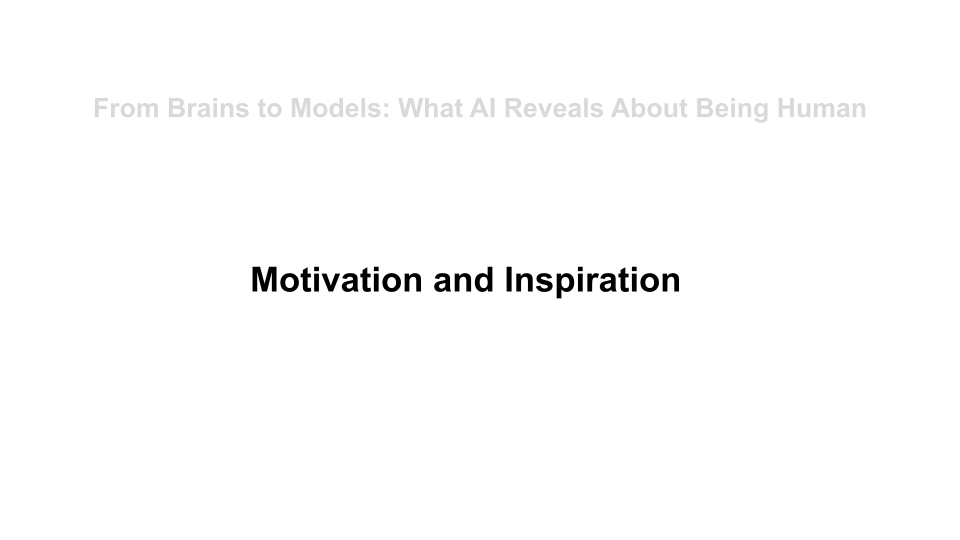
\includegraphics[width=.64\linewidth]{figures/talk/slide-02.png}}
\biopath
This divider invites you to identify a reason for learning the material. A useful starting question is: what would I need to understand before relying on an AI output in my own field? Choose an example such as identifying an enhancing lesion, following change over time, or explaining a positive screening result. List what is observed, what is inferred and what decision might follow. These are different stages, and each can fail in a different way. Image contrast can change with acquisition; a segmentation can inherit an annotation convention; an accurate probability can still leave a difficult choice.

The biomedical route begins with these meanings and then introduces the machinery needed to examine them. Predict a result before opening a notebook, inspect the result, and explain any surprise in ordinary language. For the screening example, try counting affected and unaffected people before using a formula. For the growth example, distinguish a simulated tissue state from the coloured boundary drawn around it. By the end, aim to give a colleague an explanation that includes the purpose, the evidence and one unresolved assumption. That is a stronger learning outcome than remembering a sequence of model names.
\comppath
Treat motivation as problem specification. An attractive implementation can quietly answer a different question from the one that motivated it. Write down an input, an output, an intended population and a criterion for success before choosing an architecture. Then identify the smallest runnable example that exposes the central issue. The course uses small systems because their assumptions can be inspected: fixed analytic classifiers, a trainable synthetic segmenter, an exact attention calculation, and reaction--diffusion simulations.

Distinguish three activities when using them. Demonstration shows that a phenomenon can occur under chosen conditions. Verification checks whether code implements the stated mathematics. Empirical validation asks whether the model describes observations sufficiently well for a specified purpose. A single notebook can support more than one activity, but the evidence for each must be identified separately. Start a learning log with a prediction and a possible failure criterion. After running, record the observed discrepancy and a proposed explanation. If a result agrees with your prediction, ask whether the test could have exposed a plausible bug or alternative mechanism. The computational route develops this habit alongside the calculations.
\end{slidenotes}

\begin{slidenotes}{03}{Biological brains across scales}{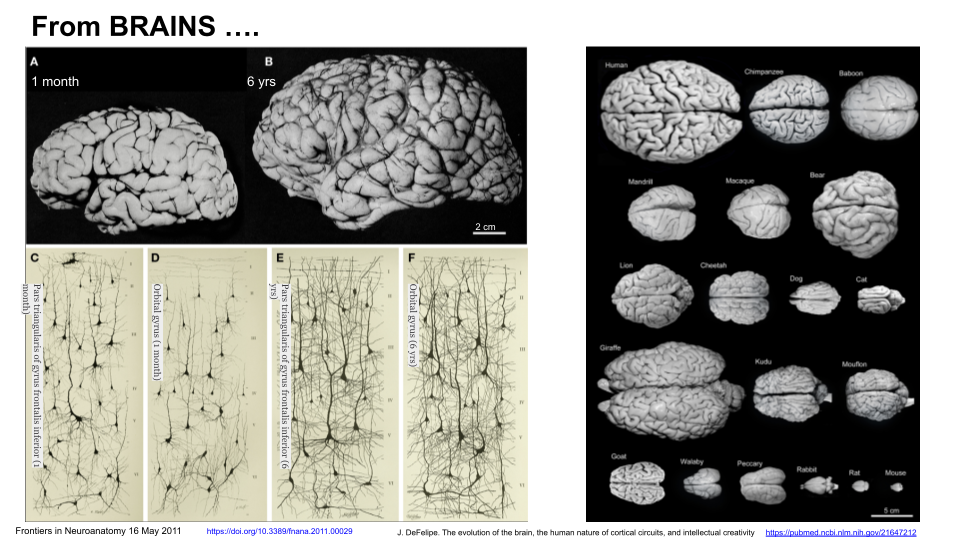
\includegraphics[width=.64\linewidth]{figures/talk/slide-03.png}}
\biopath
The slide juxtaposes cortical drawings at different developmental ages with brains from different mammals, drawing attention to biological diversity across scales. The neuron drawings concern local organisation; the whole-brain images concern macroscopic form. Their scale bars matter. A larger drawing on the page does not necessarily represent a larger biological structure. Nor does a difference in visible branching establish a difference in intelligence. Such claims would require appropriate measurements, comparable sampling and an account of development, species and behaviour.

For imaging students, this is a reminder that an MRI voxel aggregates signals from many microscopic components. A change in a macroscopic measurement may have several biological explanations. Conversely, a cellular change may occur without a detectable change in gross anatomy. Move carefully between scales: state which structure was observed, by which method, and which further process is being inferred. Brain development also includes interaction with a body and environment over time; a static anatomical panel captures only part of that history. As an exercise, choose one visible contrast in the slide and write a descriptive claim supported by the picture. Then write a mechanistic claim that would require additional data. Explain what those data would need to measure.
\comppath
The route from biology to computation begins with deciding which properties to model. A neuron can be represented by a detailed biophysical system, a firing-rate variable or a simple threshold unit, depending on the question. Each choice discards information. This is useful abstraction when the retained variables suffice for the target phenomenon; it becomes misleading when the omitted properties are needed to support the conclusion. The drawings therefore motivate a modelling decision rather than prescribe a particular artificial architecture.

Separate structural similarity from functional and causal similarity. Two networks could have comparable connection statistics yet compute different mappings. Two systems with different connectivity could produce similar answers on a restricted task. A convincing comparison needs a shared observable and a test that probes how it arises. For example, compare responses to the same controlled stimulus and then perturb a proposed pathway. \coursenotebook{03_bio_vs_artificial.ipynb}{Notebook 03} offers a supplementary comparison of learning systems; its architectures and learning rules change together, so an observed difference cannot be attributed to either factor alone. Design a hypothetical comparison that tests each learning rule in each architecture, so the two factors can be separated. This makes the limitations of an analogy informative rather than merely disappointing.
\end{slidenotes}

\begin{slidenotes}{04}{Architectures encode choices}{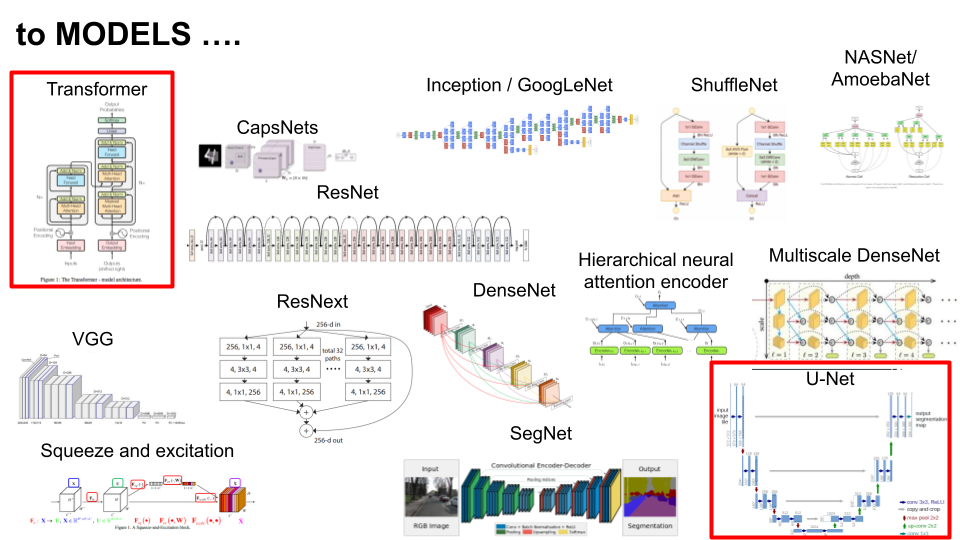
\includegraphics[width=.64\linewidth]{figures/talk/slide-04.png}}
\biopath
The architecture collage shows that there is no single design called ``the neural network''. Networks arrange computations in different ways to suit different tasks. A classifier may compress an entire image into a diagnosis-related score. A segmentation network must also preserve enough spatial information to assign labels to individual pixels or voxels. The highlighted U-Net family combines information at broader and finer spatial scales; the highlighted Transformer uses attention operations to combine information according to relationships within its input representation \citep{ronneberger2015,vaswani2017}.

For an imaging application, begin with the output needed and work backwards. Does the task require a local boundary, a whole-image category or a report? Which image contrasts and spatial relationships are available? A sophisticated architecture cannot restore information that was never measured, and a high average score can conceal failures on small lesions or unfamiliar acquisitions. Architecture names also say little about annotation policy, training population or calibration. Compare two candidate systems by asking what each sees, what it predicts, and how its errors would affect the intended use. The purpose of this slide is to recognise design choices and their implications; memorising every branch of the collage contributes much less to that judgment.
\comppath
An architecture specifies a family of functions and constrains how information flows. Convolutions reuse local filters; residual connections provide additive routes through a network; encoder--decoder structures combine spatial compression with reconstruction of an output grid. Attention computes input-dependent combinations of value vectors. These choices influence optimisation and the kinds of regularity that can be represented efficiently. Training then selects parameters within that family using a dataset, objective and optimisation procedure.

Do not infer an explanation from the diagram alone. A skip connection permits information flow, but demonstrating that a particular cue controls a prediction requires an intervention. Likewise, an attention matrix is one intermediate quantity rather than a complete account of the network's dependence on its input. Use \coursenotebook{01_tiny_transformer.ipynb}{Notebook 01} to trace a small Transformer and \coursenotebook{09_segmentation_reflection.ipynb}{Notebook 09} to inspect a trained synthetic segmentation example. Keep the output definition and evaluation examples fixed when comparing models. If several architectural and training choices change together, report the comparison as a comparison of systems. To attribute an improvement to a specific component, construct an ablation (a controlled removal or alteration of that component) and assess whether the conclusion survives relevant data shifts.
\end{slidenotes}

\begin{slidenotes}{05}{Four questions about intelligence}{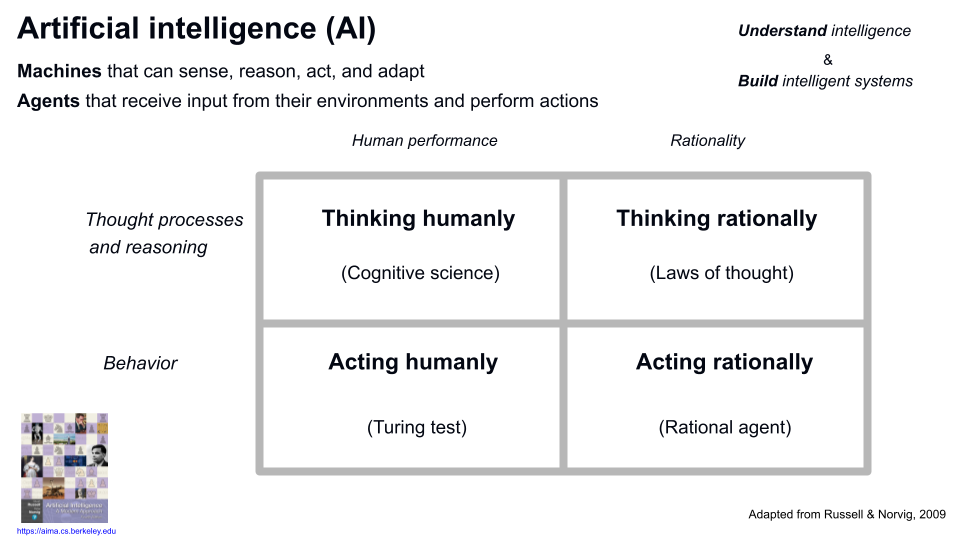
\includegraphics[width=.64\linewidth]{figures/talk/slide-05.png}}
\biopath
The Russell--Norvig grid crosses two distinctions: thinking versus acting, and human resemblance versus rational performance. Each cell asks a different question. A system can reproduce a clinician's answers, model the clinician's reasoning process, make formally consistent inferences, or select actions that serve a specified objective. These achievements can come apart. Matching a historical prescribing pattern, for example, could reproduce a systematic mistake. Following a formal rule could also be inappropriate if the rule omits an important patient concern.

Use the grid to clarify what an evaluation establishes. Agreement with an expert measures a form of behavioural resemblance. A study of response times or error patterns can contribute evidence about processing. Expected-utility analysis evaluates actions relative to stated outcomes, probabilities and preferences. Calling an action rational does not make those preferences universal or remove uncertainty. In clinical work, ask who defined the objective and whose outcomes were counted. Take a familiar diagnostic decision and place four possible research questions into the four cells. Then choose the evidence each would require. The same AI system may be relevant to all four questions, but a successful test in one cell does not answer the others.
\comppath
Translate each cell into an observable target. ``Acting humanly'' could mean that a judge cannot reliably distinguish a model's answers from human answers under a fixed protocol. ``Thinking humanly'' needs a model of process and predictions that discriminate it from alternatives. ``Thinking rationally'' might concern valid inference within a specified formal system. ``Acting rationally'' concerns action selection relative to an objective and available information. The labels become useful only when the task and success criterion are explicit.

\coursenotebook{04b_four_views_of_AI.ipynb}{Notebook 04b} treats the grid as a catalogue of evaluation questions. It does not supply a measured verdict on a named model. Use it to identify a common category error: optimising agreement with human labels and then claiming optimal decisions. A classifier trained to minimise prediction loss does not automatically minimise the downstream cost of acting. Conversely, a decision policy can be useful while producing explanations unlike human reasoning. For an exercise, define separate metrics for human agreement and expected decision cost on the same constructed cases. Work out a case in which the metrics rank two systems differently. The disagreement identifies the extra assumptions needed to choose between them.
\end{slidenotes}

\begin{slidenotes}{06}{Embodiment, judgment and collaboration}{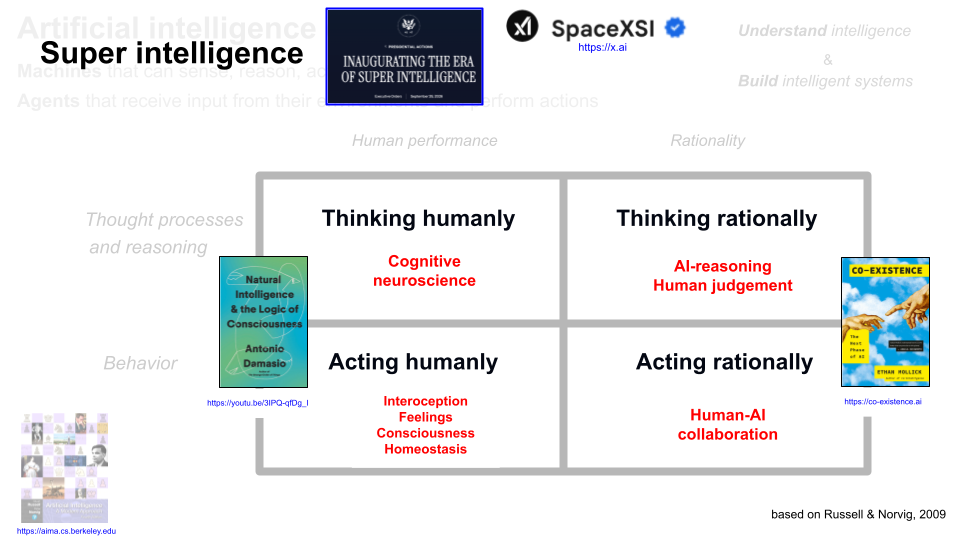
\includegraphics[width=.64\linewidth]{figures/talk/slide-06.png}}
\biopath
The annotated grid extends the previous slide towards cognitive neuroscience, judgment, feelings and collaboration. Interoception concerns signals about the body's internal condition; homeostasis concerns regulation that keeps physiological variables within viable ranges. These processes help explain why biological cognition is bound to needs, action and a continuing life. Their presence in the discussion motivates questions about embodied understanding. It does not supply a simple anatomical test for consciousness or a proof that one particular mechanism is sufficient for experience \citep{seth2013,sethbayne2022}.

In medicine, collaboration can be evaluated even when these philosophical questions remain open. Consider an AI-drafted explanation of a scan. Its wording may be fluent while the clinician must still recognise uncertainty, respond to distress and connect the explanation to the patient's circumstances. Assess the combined interaction: what information was conveyed, what the patient understood, and what responsibility the professional exercised. The books and headlines on the slide are prompts for discussion rather than experimental evidence. Choose one claim, such as ``this system understands the patient's concern'', and specify a narrower observation that could be tested. Then identify what would remain uncertain even if that observation were positive.
\comppath
A regulated software system can monitor variables, maintain constraints and pursue goals. These functional properties are worth describing precisely. They do not by themselves settle whether its states have the biological or experiential significance of hunger, pain or concern. Keep functional terms tied to an operation: a controller reduces an error signal; an agent selects tool calls; a language model produces a context-dependent continuation. Moving from an operation to a claim about subjective experience requires a further argument and evidence.

Human--AI collaboration introduces another unit of analysis: the coupled system of model, interface, professional and environment. Measure whether assistance improves performance under the actual division of labour. Useful comparisons include unaided judgment, unaided model output and the combined workflow, with the same cases and outcome definition. Examine whether assistance changes error detection or encourages inappropriate agreement. Appendix~\ref{app:4e} develops embodied, embedded, enactive and extended perspectives as questions that can guide such studies. As a computational exercise, describe a feedback loop and identify the state variables that belong to the software, the user and the environment. This makes the brain analogy specific enough to investigate without allowing the analogy to stand in for evidence.
\end{slidenotes}

\begin{slidenotes}{07}{What a Turing-like test measures}{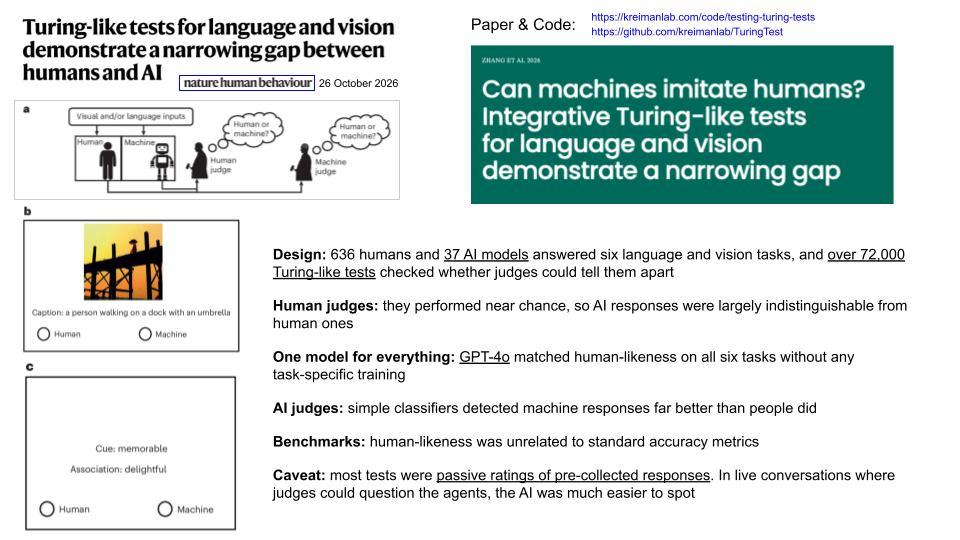
\includegraphics[width=.64\linewidth]{figures/talk/slide-07.png}}
\biopath
The displayed study examines whether judges can distinguish human from machine responses on specified language and vision tasks. It is a test of detectable human resemblance under a protocol. In the published version, 636 human contributors and 37 AI models supplied responses; 72,191 refers to judgment trials, not independent participants. Near-chance discrimination in some conditions does not imply that all models passed every task \citep{zhang2026turing}.

An everyday clinical analogy helps separate the questions. A machine-written report may sound convincingly human while containing an incorrect measurement. A terse, recognisably automated output may contain the correct measurement. Humanness, accuracy and usefulness therefore need separate assessments. A judge may also rely on a superficial cue, such as habitual wording, rather than the quality of the reasoning. Suppose an apparently human report contains a subtle contradiction between the findings and conclusion. What would a source-identification test reveal, and what would a clinical review reveal? Use the distinction to design two evaluation forms: one asks who produced the report; the other checks its factual and interpretive content. Neither should be used as a substitute for the other. The slide invites an operational question about behaviour, while leaving mechanisms and experience open.
\comppath
Treat source identification as a classification problem. Specify the sampling of human and model answers, information available to the judge, class balance and metric. Fifty per cent accuracy is a chance reference for a balanced binary task, but a confusion matrix reveals whether the judge systematically favours one source. Repeated judgments about the same answer are dependent observations; uncertainty estimates should respect the sampling structure rather than count every click as a new independent response.

Separate answer quality from detectability by measuring both on the same items. A model could become harder to identify by reproducing human mistakes, so improved imitation need not indicate improved task performance. Similarly, a detector can exploit a collection artefact that disappears in a new setting. Hold out stimuli or participants as appropriate and ask whether source-specific preprocessing creates unintended cues. The authors also evaluate AI judges; comparisons require attention to differences in training and task conditions. For a small exercise, create responses with an irrelevant formatting cue correlated with source. Compare a detector before and after the cue is removed. A large performance drop would diagnose a property of the benchmark construction rather than a general ability to recognise machine reasoning.
\end{slidenotes}

\begin{slidenotes}{08}{Read results in their time and protocol}{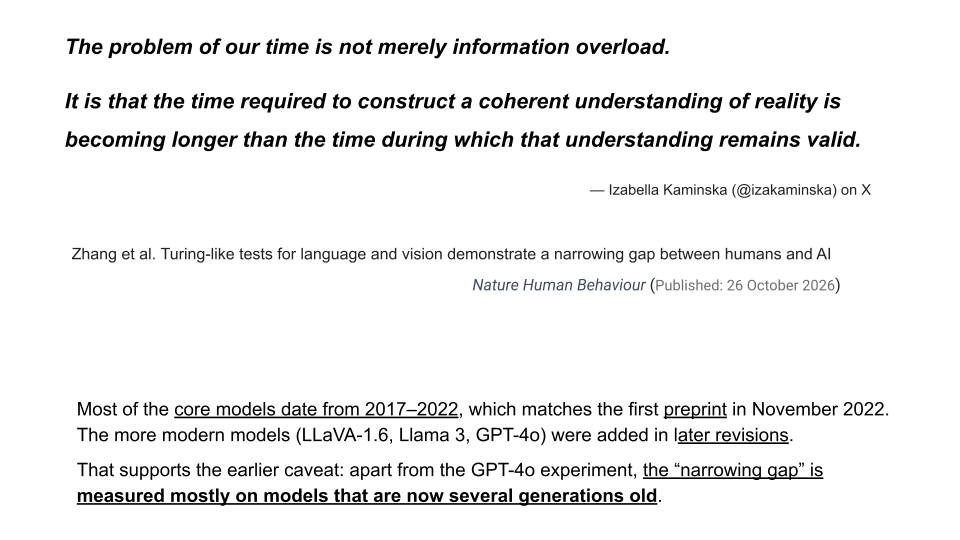
\includegraphics[width=.64\linewidth]{figures/talk/slide-08.png}}
\biopath
The quotation on the slide encourages scrutiny of a study's continuing relevance. A publication date and a model's release date answer different questions: when evidence appeared and which system was tested. Findings about an older system remain evidence about that system and setting. Applying them to a newer tool requires an additional comparison. The published Turing-like study also includes Claude 3.7 and LLaMA 3.3 conversation experiments, so the thumbnail's emphasis on older models is incomplete \citep{zhang2026turing}.

For clinical readers, think of a diagnostic assay that changes between study and deployment. Evidence is neither automatically obsolete nor automatically transferable. Identify what changed: the instrument, instructions, sampled population or outcome definition. An updated language model could improve factual responses while becoming easier to recognise, or the reverse. The original study can still offer a useful protocol, error taxonomy or comparison baseline. Write a short appraisal with three sentences: what was actually measured, which features of your intended use match that setting, and which difference requires new evidence. This practice avoids turning a debate about the age of technology into a vague verdict on an entire paper. It also makes a replication question sufficiently precise to answer.
\comppath
Version is part of the experimental specification. Record the model identifier, access date, system instructions, generation settings and input preprocessing alongside the evaluation code. A name that refers to a changing service is weaker provenance than a fixed snapshot. Where exact replay is unavailable, save permissible inputs and outputs and describe the limits of repeatability. These records allow a later researcher to separate a changed system from a changed measurement procedure.

The published study distinguishes passive assessment of existing responses from interactive questioning. Those protocols provide different information to a judge; changes in models and instructions also prevent treating every difference as an isolated effect of interactivity. To investigate one factor, hold the others fixed where possible. A useful replication matrix crosses model version with protocol, using matched tasks and explicit human sampling. Predefine the source-identification metric and a separate task-quality score. Do not tune the prompt on the final evaluation items. Finally, state whether the replication tests a historical result, an updated capability or transfer to a clinical task. Each objective supports a useful experiment, but combining them without a design makes a changed score difficult to interpret.
\end{slidenotes}

\begin{slidenotes}{09}{Turn a model suggestion into a study}{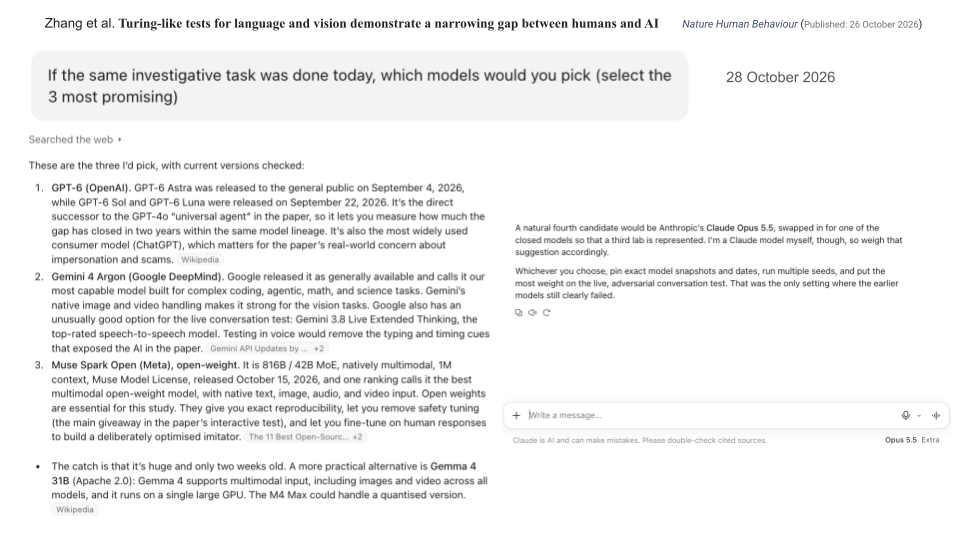
\includegraphics[width=.64\linewidth]{figures/talk/slide-09.png}}
\biopath
This slide shows an AI-generated proposal for choosing contemporary models to revisit the preceding study. Read it as a draft research suggestion. A confident list of names and capabilities is not a completed comparison, and the screenshot supplies no performance evidence for the proposed systems. The first educational task is to turn the suggestion into a question: are we testing human resemblance, answer accuracy, or suitability for a particular clinical activity?

Choose a clinically intelligible task before choosing a favourite model. For example, ask whether a short explanation preserves uncertainty and agrees with a supplied imaging report. Define what a human comparison group receives and what the judges are allowed to inspect. Include experts when factual adequacy requires domain knowledge; a general reader can judge clarity but may miss a subtle diagnostic error. Decide in advance what would count as improvement and what kind of error would be unacceptable for the proposed use. A small pilot can expose ambiguous instructions, but pilot cases should not silently become the final test set. The value of the suggestion is therefore its capacity to initiate a disciplined comparison. Its persuasive presentation should not determine the conclusion.
\comppath
Convert the screenshot into a reproducible protocol. First verify that each candidate system exists, is accessible and supports the required input modality at the time of the experiment. Record exact versions and settings instead of treating the proposed list as a current recommendation. Next define shared inputs, allowed tools, response limits, parsing rules and handling of failed or incomplete outputs. Differences in tool access or context can otherwise masquerade as differences between base models.

Separate protocol development from evaluation. Use development items to resolve formatting and instructions, then freeze the procedure before testing held-out stimuli. Repeated runs estimate variability under the chosen generation settings; report that variability alongside the human sampling uncertainty. Inspect whether multiple judgments or outputs share the same underlying item, and analyse the corresponding dependence. Include a straightforward baseline so that elaborate prompting must justify its added complexity. Save a failure log with examples and explanations that can be checked independently. Finally, distinguish a prospective design from measured results in every table and caption. This exercise illustrates a productive use of AI in research: generating a candidate plan whose assumptions, feasibility and conclusions are then examined by the investigator.
\end{slidenotes}

\begin{slidenotes}{10}{From patient data to a useful decision}{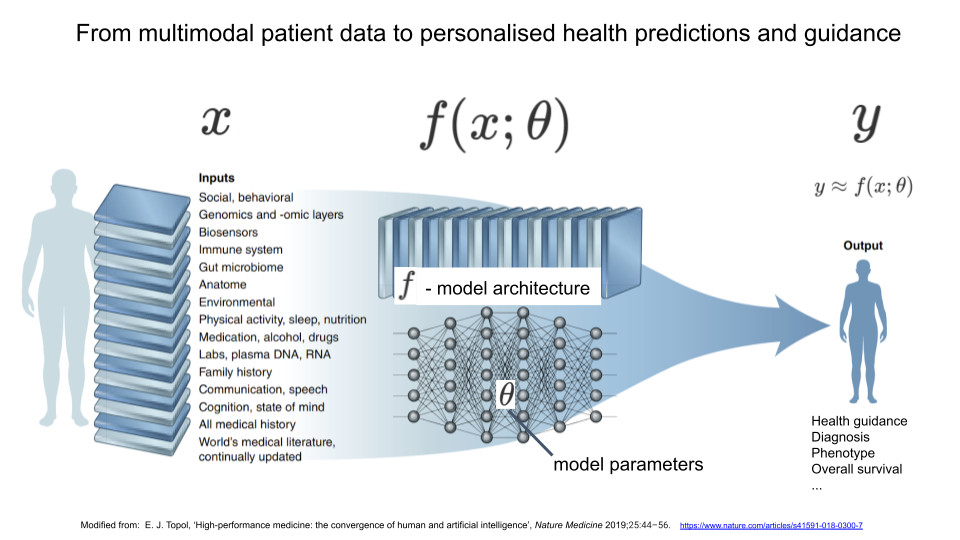
\includegraphics[width=.64\linewidth]{figures/talk/slide-10.png}}
\biopath
The diagram brings together measurements such as images, molecular data and clinical information as inputs to a model, which produces an output relevant to care. The notation $x\mapsto f(x;\theta)\mapsto y$ compresses a long chain. Someone decides what to measure, aligns records, defines an outcome and chooses how a predicted quantity enters practice. A probability of progression, an anatomical label and a treatment recommendation have different meanings and require different evidence.

Consider predicting an outcome at the time of a scan. Only information available then belongs in the intended prediction setting. A later investigation or a note written after the outcome can make retrospective accuracy look impressive while being unavailable when needed. Missing measurements can also carry information about referral and clinical practice rather than disease alone. Ask when each input was obtained and why it exists. Then distinguish prediction from action: an estimated risk does not specify how a patient values treatment burdens. Section~\ref{sec:decisions} and \coursenotebook{15_ppv_and_decisions.ipynb}{Notebook 15} show why prevalence and stipulated consequences matter. A useful explanation of this diagram should therefore connect the patient, measurement process, predicted quantity and decision, rather than stop at the central model box.
\comppath
Here $x$ denotes the input representation, $\theta$ the fitted parameters and $y$ the target or predicted output, depending on the diagram's convention. Make that last distinction explicit in implementation: a reference outcome and an estimate of it are separate objects. Multimodal learning also requires an alignment rule. Images, laboratory results and notes must refer to the appropriate person and time; otherwise the apparent benefit of combining modalities can arise from leakage or mismatched sampling.

Evaluate the full pipeline, including preprocessing and missing-data handling, using patient-level separation where patients contribute repeated records. A held-out hospital or later time period can probe transfer beyond the development setting. Assess calibration when predicted probabilities will support decisions, and measure clinically relevant error patterns as well as aggregate discrimination. A model estimating outcomes under observed care does not automatically estimate the effect of changing treatment: treatment selection and confounding enter that causal question. \coursenotebook{11_shortcut_dependence.ipynb}{Notebook 11} provides a controlled illustration of reliance on constructed cues using fixed analytic rules. Use it to formulate an intervention on an irrelevant input feature before claiming that a multimodal representation has learned the intended biological relationship.
\end{slidenotes}

\begin{slidenotes}{11}{Keep the task fixed across Marr's levels}{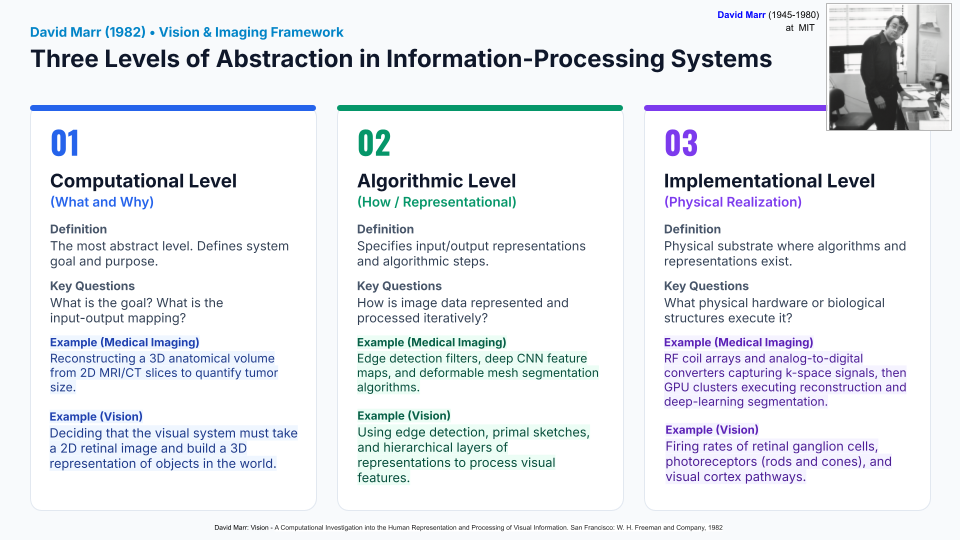
\includegraphics[width=.64\linewidth]{figures/talk/slide-11.png}}
\biopath
Marr separates an explanation of what a system does and why, an account of its representations and algorithms, and its physical implementation \citep{marr2010}. Keep one task fixed to see the distinction. Suppose the aim is to compare the spatial extent of enhancing tissue across two examinations. At the computational level, define that target and explain why measuring it is useful. At the algorithmic level, describe how an image becomes a mask and how the mask becomes a volume. At the implementation level, identify the hardware that stores the data and executes those operations.

A simple volume calculation makes this tangible. If a mask contains 1,000 voxels and each voxel occupies 2~mm$^3$, the represented volume is 2,000~mm$^3$, or 2~mL. This calculation can be exact even when the mask boundary is uncertain or enhancement is an imperfect marker of the biological quantity of interest. The slide ranges across acquisition, reconstruction and segmentation; in discussion, avoid switching among them unnoticed. MRI reconstruction estimates an image from acquired signals, while segmentation assigns labels to an image. Choose one of these tasks before filling in the three columns. The framework then helps locate a disagreement rather than merely rename it.
\comppath
For the fixed lesion-volume task, specify the input image and target convention first. A possible representation is a binary array $m_i\in\{0,1\}$ with voxel volumes $v_i$; an algorithm computes $V=\sum_i m_iv_i$. The mask itself may come from manual annotation, a convolutional network or another procedure. Those alternatives share a downstream calculation while differing in how they obtain its inputs. The physical realisation includes memory, processors and numeric representations used to execute the chosen procedure.

Different levels constrain one another without being interchangeable. Available memory can restrict image resolution, which can affect the accuracy of a boundary estimate. Yet identifying a GPU does not establish that the segmentation policy is appropriate. Likewise, agreeing on the clinical purpose does not specify a correct algorithm. In MRI, radiofrequency signals are sampled in a measurement domain often described through k-space; a stack of reconstructed slices is already a processed representation. Keep these stages distinct when describing the implementation examples on the slide. \coursenotebook{00_intro_timeline.ipynb}{Notebook 00} offers a starting exercise. For a proposed improvement, identify which level changes and which observation would demonstrate its benefit. Explicit clinical context accompanies all three levels; it is not a fourth level in Marr's original framework.
\end{slidenotes}

\begin{slidenotes}{12}{Read about AI with an application in mind}{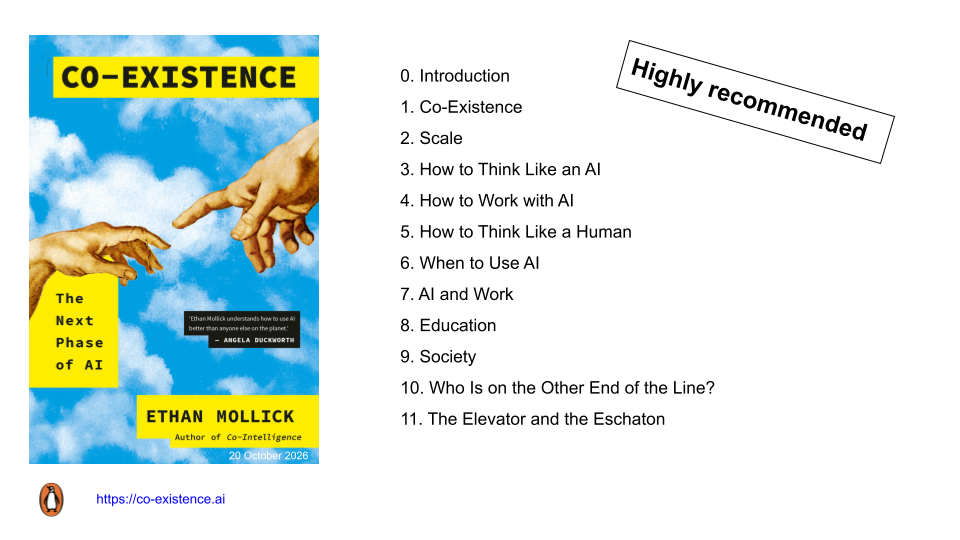
\includegraphics[width=.64\linewidth]{figures/talk/slide-12.png}}
\biopath
The book recommendation marks a move from comparing systems to learning how to work with them. Mollick's \emph{Co-Existence} spans AI capabilities, human thinking, work, education and society \citep{mollick2026coexistence}. Use that breadth to generate questions relevant to your own practice. A chapter about education, for example, can prompt a distinction between completing an assignment and acquiring the ability to solve the next problem unaided. A chapter about work can prompt an examination of how verification effort changes when drafting becomes easier.

Read actively rather than treating a recommendation as a settled account of every domain. Select one claim, identify the setting in which it might apply, and ask what evidence would support transfer to biomedical work. A tool that helps brainstorm a patient-information leaflet still needs checking for factual accuracy, audience understanding and suitability for the situation. Keep a short reading note with a claim, a concrete example and a testable implication. Then compare your interpretation with someone taking the other path. The aim is to connect a broad account of technological change to a carefully bounded learning or research task. The book is a discussion resource; the particular application supplies the evaluation question.
\comppath
Use the table of contents as a map of levels at which an AI system can be studied: model behaviour, user interaction, organisational workflow and social consequences. A performance benchmark concerns a different unit of analysis from a study of whether a team becomes more effective. The same underlying model can support very different outcomes depending on the interface, instructions, checks and division of labour. Define that surrounding system before comparing productivity claims.

For a small study, choose a task with a checkable output, such as extracting a fixed set of fields from supplied reports. Measure accuracy, completion time and review time separately. Record corrections and unresolved cases rather than counting every generated field as completed work. If the goal is learning, add a later unaided task; if the goal is workflow improvement, include the cost of detecting errors. These choices allow a clear comparison between immediate output and retained competence. Make explicit which parts of the procedure come from your own design and which are hypotheses inspired by the reading. A general book can help formulate useful questions, while a reproducible protocol determines what your experiment can establish about a specific tool and context.
\end{slidenotes}

\begin{slidenotes}{13}{Preserve the ability to judge}{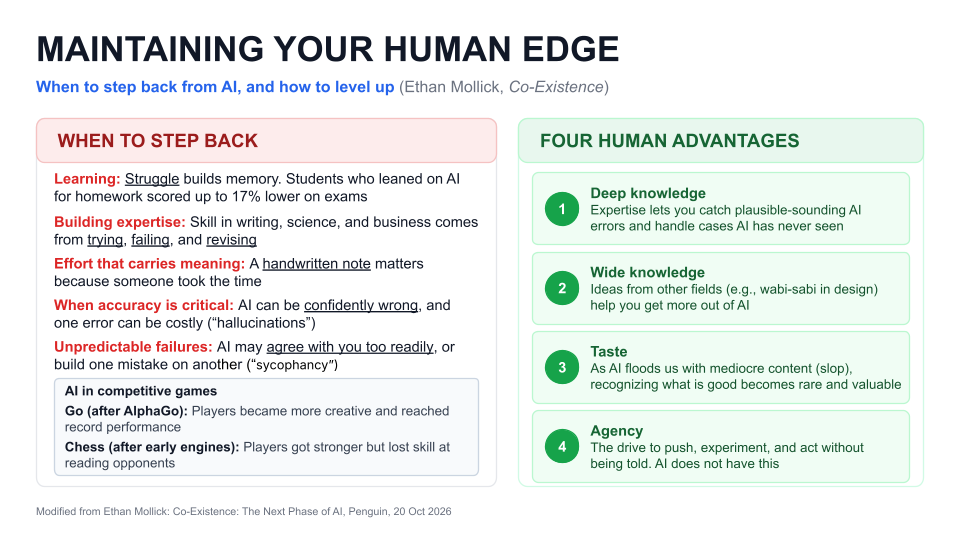
\includegraphics[width=.64\linewidth]{figures/talk/slide-13.png}}
\biopath
The slide asks when assistance strengthens your work and when it removes the practice needed to become competent. Its examination statistic refers to a particular high-school mathematics experiment: the unrestricted GPT-4 group scored 17\% lower than the control group when assistance was removed; a tutor designed with learning safeguards largely mitigated that effect \citep{bastani2025learning}. This is not a universal effect size for AI use, university students or medical education. It illustrates why assisted performance and subsequent independent learning should be measured separately.

Hallucination is plausible but unsupported content; sycophancy is inappropriate agreement with the user. In imaging education, try describing a scan or checking a volume calculation yourself before viewing an AI answer. Then compare the explanations, identify the discrepancy and solve a related case without assistance. Asking for a hint can preserve more of this work than requesting a finished answer. The slide's proposed human strengths---depth, breadth, taste and agency---can be translated into practice: know enough to detect an error, connect ideas across fields, justify a quality judgment and take responsibility for a choice. Treat its game-playing examples as discussion prompts rather than evidence of a general educational law. The central question is whether a particular pattern of tool use develops or bypasses the competence you are trying to acquire.
\comppath
When studying assistance, choose outcomes that distinguish output production from skill acquisition. Immediate accuracy, review accuracy and delayed unaided transfer are different variables. A learner can complete more tasks with a tool while becoming less able to diagnose a new failure independently. Randomised assistance conditions and common unaided assessments can help identify that distinction. Preserve the task difficulty and scoring rule across groups, and account for the possibility that users respond differently to direct answers and guided hints.

The slide's statement about agency also needs a precise reading. Software agents can select actions and pursue assigned objectives; this is a functional property that can be implemented and tested. The broader claim concerns self-originated human motivation, meaningful commitments and responsibility, which are not established merely by observing a sequence of tool calls. Describe the operational capability before drawing a philosophical conclusion. As an exercise, inspect an AI-produced solution that contains one subtle unit error. Record whether you can find and explain it before running a checker. Then design assistance that supports diagnosis without immediately revealing the correction. A useful learning system should make the student's reasoning more inspectable and transferable, not only increase the number of plausible answers on the page.
\end{slidenotes}

\begin{slidenotes}{14}{Map the frontier task by task}{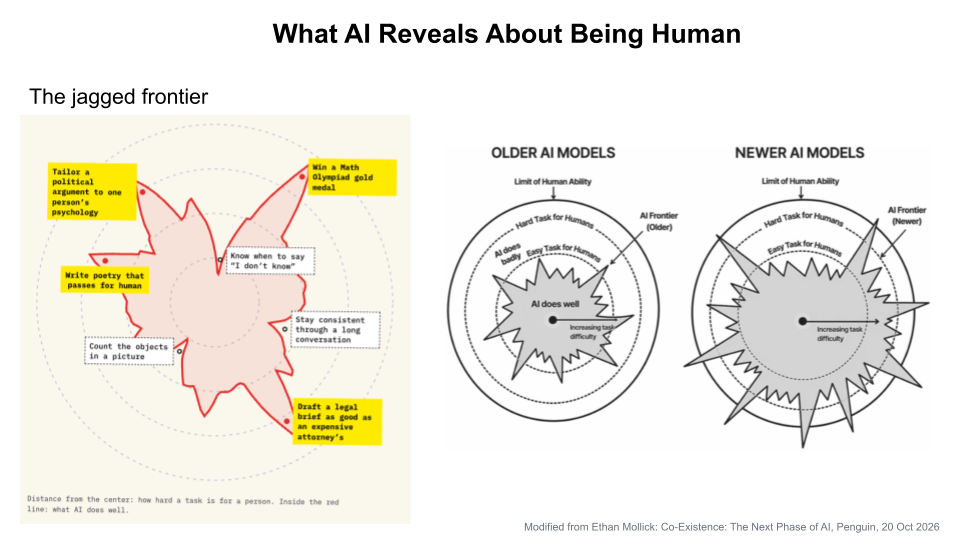
\includegraphics[width=.64\linewidth]{figures/talk/slide-14.png}}
\biopath
The jagged boundary represents uneven capability: a system may perform well on a task people find difficult yet fail on a task people find easy. The diagrams are conceptual illustrations, not measured maps of a clinical tool \citep{mollick2026coexistence}. Their radial arrangement should not be read as a calibrated scale of intelligence. The useful message is that intuition about human difficulty offers an unreliable guide to the reliability of an unfamiliar AI system.

Apply this to an imaging workflow. A model might produce a fluent summary yet mishandle a small numerical comparison, laterality or the timing of an examination. Conversely, it might identify a subtle image pattern consistently while failing to explain its significance. These are candidate failure modes to test, not conclusions supplied by the diagram. Break the workflow into observable operations and evaluate each on representative cases. Include uncommon but consequential situations rather than relying entirely on average performance. If a system changes, repeat the relevant checks instead of assuming that every capability improves together. The practical exercise is to draw your own evidence map: put a task, its observed errors and its tested conditions beside each point. Leave untested territory explicitly unmeasured.
\comppath
A capability frontier depends on model version, prompting, tool access, data distribution and the chosen success threshold. It is therefore a property of an evaluation setting as well as a model. Replace the sketch with a table of tasks and measurable criteria. For each task, report the number and source of examples, the metric, uncertainty and observed failure modes. A boundary inferred from a handful of demonstrations is likely to move when the input distribution changes.

Avoid selecting only examples that confirm a preferred picture. Use a development set to formulate the task categories and an independent test set to estimate performance. If an agent can retry or use tools, include those resources in the protocol and cost comparison. Compare the same tasks across system versions rather than comparing different benchmark collections. A regression on one operation can matter even when an aggregate score rises. \coursenotebook{11_shortcut_dependence.ipynb}{Notebook 11} supplies a small example of how changing a cue relationship can alter the ranking of fixed classifiers. Use it to explain why capability under one distribution does not establish robustness under another. The operational counterpart of the jagged sketch is a maintained set of relevant tests, including the failures that motivated them.
\end{slidenotes}

\begin{slidenotes}{15}{Specify, inspect, revise and stop deliberately}{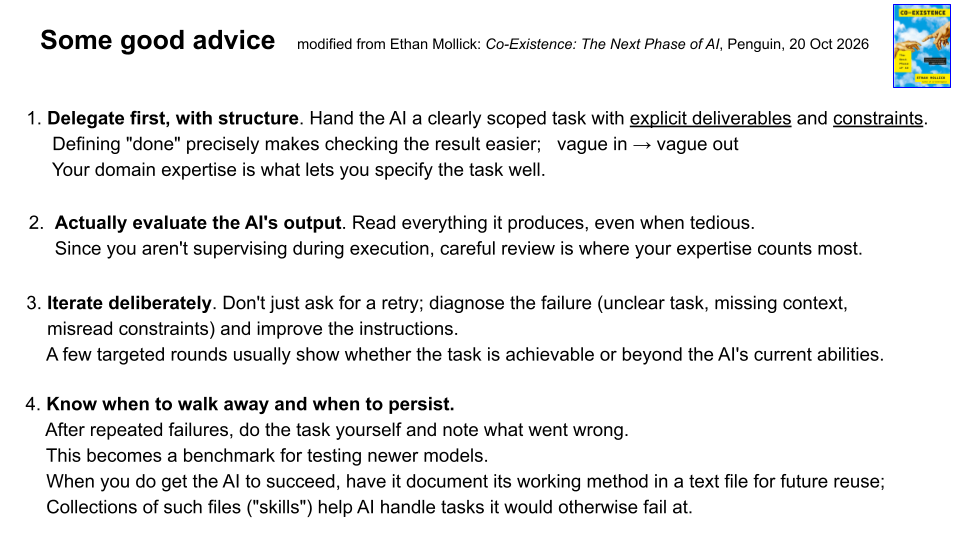
\includegraphics[width=.64\linewidth]{figures/talk/slide-15.png}}
\biopath
The four recommendations turn collaboration into a sequence you can inspect: define a bounded task, examine the result, diagnose the failure and decide whether further work is worthwhile. Consider asking for an explanation of a segmentation result. Specify the intended audience, the supplied evidence and the distinction between an image finding and a biological interpretation. A useful deliverable might be a short explanation that preserves uncertainty and defines the unfamiliar terms. You can then assess whether the result meets those requirements.

Evaluation must include the content that a polished answer makes easy to overlook. Check numbers against the source, follow citations to the actual passage, and ask whether the conclusion goes beyond the observations. If a term was misunderstood, revise that part of the instructions and retain the failed example for comparison. Repeated confident errors suggest that more prompting may be less useful than doing the task directly or consulting an appropriate source. When a procedure works, document the inputs and checks that made it work. A reusable method should help the next user recognise a failure as well as reproduce a success. This is a practical interpretation of the advice on the slide, adapted to accountable biomedical work.
\comppath
Express the task as an input--output contract with acceptance criteria. For a simulation request, specify the equation, units, boundary conditions, parameters and outputs before requesting code. Then use independent checks: a spatially uniform solution, a conservation property or a comparison with a trusted limiting case. Successful execution and attractive plots are weak evidence if no test could distinguish the intended model from a plausible incorrect implementation. \coursenotebook{13_verified_growth_model.ipynb}{Notebook 13} demonstrates several stronger checks.

Iteration should be diagnostic. Preserve the failing input, error and expected behaviour; change the suspected cause; then rerun the relevant check. Changing many instructions simultaneously can repair an output while obscuring what was wrong. A model-generated explanation of its own success is a hypothesis to investigate, not an independent verification. Define a stopping rule in terms of unresolved errors, available evidence and the cost of further attempts. Save a working method with its environment, dependencies and known limits so that another person can use it. This makes the slide's practical advice testable and supports a useful division of labour: AI can propose and implement, while acceptance rests on explicit criteria and evidence that can be examined outside the generation process.
\end{slidenotes}

\begin{slidenotes}{16}{Compartments, anatomy and measurement}{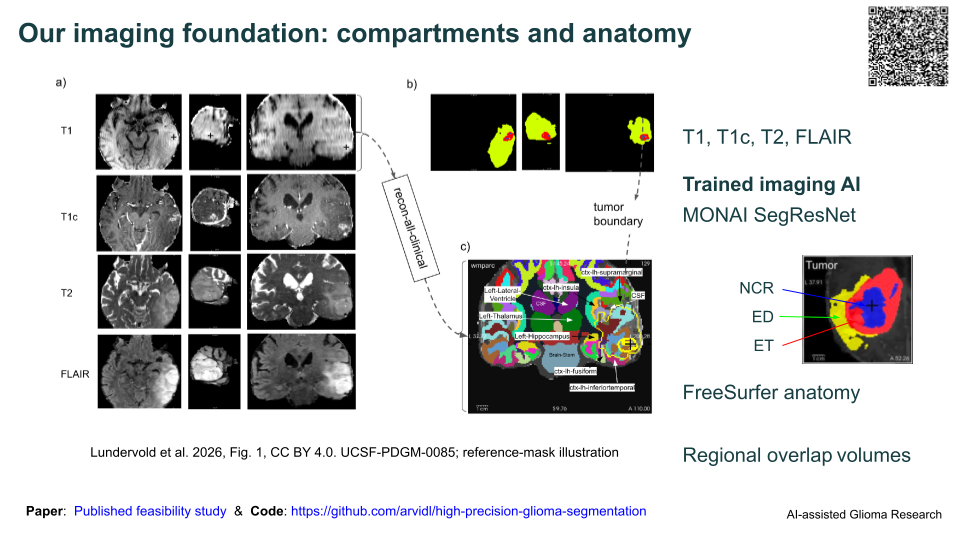
\includegraphics[width=.64\linewidth]{figures/talk/slide-16.png}}
\biopath
The multiparametric MRI panel combines T1-weighted images, contrast-enhanced T1 (T1c), T2-weighted images and fluid-attenuated inversion recovery (FLAIR). T1c emphasises contrast enhancement; T2 and FLAIR reveal different water-related signal changes, with FLAIR suppressing cerebrospinal-fluid signal. In the displayed compartment convention, NCR denotes a necrotic/non-enhancing core category, ED an oedema-related region, and ET enhancing tumour. They are imaging label categories; their boundaries are not direct microscopic maps of every viable tumour cell. Enhancement and surrounding signal changes require interpretation in their clinical context.

The slide links those compartments to anatomical regions obtained with FreeSurfer, enabling overlap volumes. For example, the amount of a labelled lesion region inside an anatomical parcel answers a spatial measurement question. It does not alone establish functional impairment or identify infiltrating cells beyond the visible abnormality. The displayed compartment panel uses reference masks from the published feasibility study, credited in the thumbnail; it should not be read as a newly computed SegResNet prediction \citep{lundervold2026glioma}. When discussing a volume, name the compartment, anatomical coordinate system and annotation convention. Ask how partial volume, registration errors or a different labelling policy could alter the number. This connects a visually convincing overlay to the practical work required for a defensible measurement.
\comppath
Trace two outputs that are combined in the figure: a tumour-compartment segmentation and an anatomical parcellation. An overlap calculation requires both to occupy the same physical coordinate frame. Matching array dimensions is insufficient; orientation, voxel spacing and image-to-world transforms matter. For masks $m_i$ and $a_i$ on a common grid, the intersection volume is $\sum_i \mathbf{1}[m_i=1\land a_i=1]v_i$. Resampling labels generally requires a method that preserves discrete categories rather than inventing intermediate class values.

Evaluate the segmentations and the derived measurements separately. A modest boundary discrepancy can matter substantially for a small compartment or a regional overlap. Also distinguish a reference annotation from biological ground truth: agreement measures consistency with the reference policy. The slide identifies MONAI SegResNet as trained imaging AI, while \coursenotebook{09_segmentation_reflection.ipynb}{Notebook 09} is a separate synthetic exercise with a tiny NumPy model. Its controlled labels and interventions support teaching about dependence and policy; they do not reproduce the research system's patient results. For an exercise, translate one mask by a voxel and recompute regional overlap. Compare how much the total compartment volume and the intersection change. The difference demonstrates why registration quality belongs in the measurement pipeline.
\end{slidenotes}

\begin{slidenotes}{17}{Population growth and a mechanistic hypothesis}{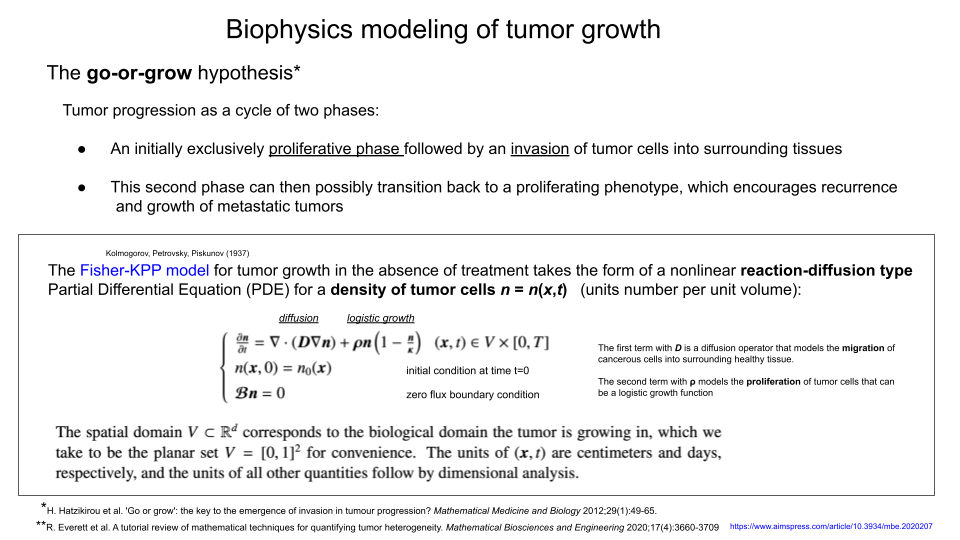
\includegraphics[width=.64\linewidth]{figures/talk/slide-17.png}}
\biopath
The equation combines spatial dispersal with local growth. A cell-density field says how many cells are represented per unit volume at each location. The dispersal term smooths density differences, while logistic growth slows as density approaches a chosen carrying capacity. These are population-level approximations. They can illustrate an advancing infiltrative pattern without tracing individual cells or resolving blood vessels and tissue microstructure.

The go-or-grow hypothesis concerns a possible trade-off between migration and proliferation, potentially involving changing cellular states \citep{hatzikirou2012}. The slide's wording about two phases should not be read as a compulsory, globally synchronised sequence. The displayed Fisher--KPP equation has one density variable and includes dispersal and growth simultaneously; it contains no explicit phenotype switching. Its mention of metastatic growth is also broader than the intended local glioma-invasion example. Keep the biological hypothesis distinct from what the equation actually implements. In \coursenotebook{14a_growth_density_and_thresholds.ipynb}{Notebook 14a}, change a display threshold while leaving the simulated state fixed. The visible boundary moves even though the underlying density does not. This is an important bridge to imaging: a thresholded outline is an observation convention, whereas a mechanistic claim concerns the process generating the state.
\comppath
Write the model as $\partial_t c=\nabla\!\cdot(D\nabla c)+\rho c(1-c/K)$, with initial density $c(\mathbf{x},0)=c_0(\mathbf{x})$ and a zero-flux boundary. If distance is measured in millimetres and time in days, $D$ has units mm$^2$/day, $\rho$ has units day$^{-1}$, and $c$ and $K$ share density units. Every term then has units of density per day. The slide's spatial-unit convention differs from the local notebooks; numerical parameter values must follow their units.

A no-flux boundary prevents transport across the domain boundary; it does not prevent the reaction term from increasing total burden. With growth disabled, a conservative discretisation should preserve integrated density. With diffusion disabled and uniform initial density, the analytic logistic solution provides another check. \coursenotebook{13_verified_growth_model.ipynb}{Notebook 13} uses these limiting cases and refinement checks to test the implementation. They verify properties of the numerical model, while evidence for glioma biology requires observations and a measurement model. If go-or-grow switching is the research target, introduce explicit states and exchange terms, specify their biological interpretation, and derive tests of that extended system. Renaming a diffusion coefficient is insufficient to add the missing mechanism.
\end{slidenotes}

\begin{slidenotes}{18}{An interactive simulation is an experiment}{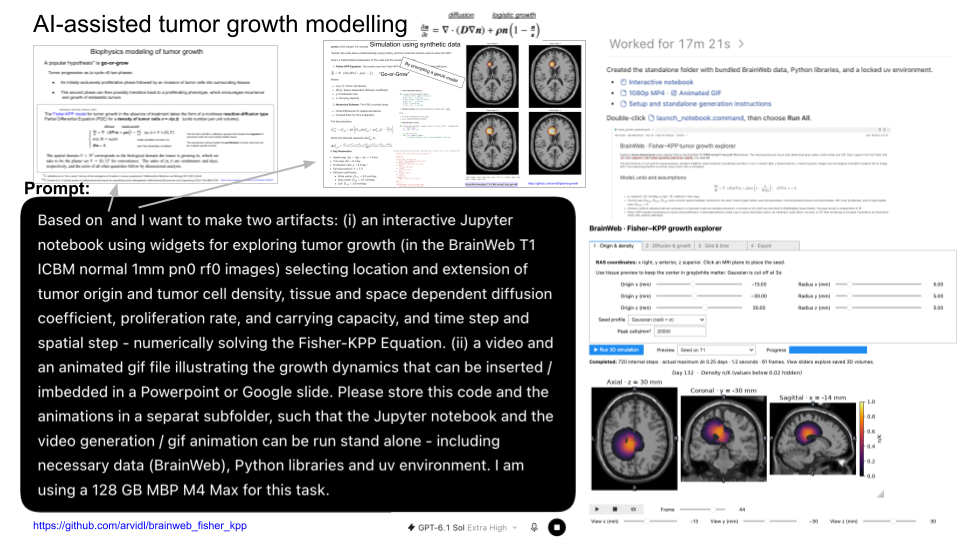
\includegraphics[width=.64\linewidth]{figures/talk/slide-18.png}}
\biopath
The prompt asks AI to build an interactive growth model in a BrainWeb anatomical image and to export an animation. The resulting interface makes assumptions manipulable: starting location, seed size, dispersal, proliferation and time can be varied. This is useful for learning because a predicted consequence can be compared with a simulated result. However, the normal BrainWeb brain is an anatomical phantom. The tumour field is generated by the model; it is not a tumour observed in that brain.

Use \coursenotebook{14b_brainweb_growth.ipynb}{Notebook 14b} for the self-contained course version. Before running, predict which tissue regions the chosen coefficients will make easier to traverse. Then change one assumption and compare matched times and display settings. Ask separately how the density changes and how a visible outline changes. A larger coloured region could reflect greater density, a lower threshold or a more permissive display. A more realistic-looking background does not turn assumed dynamics into patient-specific evidence. Record the anatomical source, model parameters and displayed quantity when sharing an animation. This preserves its value as an experiment on a mathematical model while making clear what additional observations would be needed to study an actual patient's progression.
\comppath
The prompt mixes scientific specification, software engineering and media production. Decompose it into a solver with testable inputs and outputs, an interface that changes parameters, and a renderer that reads saved states. The solver should work without the widgets. Cached states should allow slice, threshold and time controls to update displays without silently rerunning a different simulation. Exported animations should record the same parameter settings and states shown interactively.

The local BrainWeb lesson uses a density fraction $u=c/K$ and tissue-dependent scalar diffusivity. Scalar white/grey matter differences do not implement directional diffusion along fibre tracts. Physical voxel spacing and orientation must enter the calculation; coarser sampling can remove narrow barriers. Explicit time steps also need a stability bound that reflects grid spacing and diffusion. The course interface rejects unstable requested steps and distinguishes pending parameter changes from displayed cached states. Inspect these behaviours before interpreting an animation. As an exercise, keep the physical seed definition fixed while changing the grid, then compare integrated density and spatial spread. Explain which discrepancies plausibly arise from discretisation and which arise because the sampled anatomy itself has changed. This is more informative than checking whether both movies look smooth.
\end{slidenotes}

\begin{slidenotes}{19}{From a biological diagram to coupled variables}{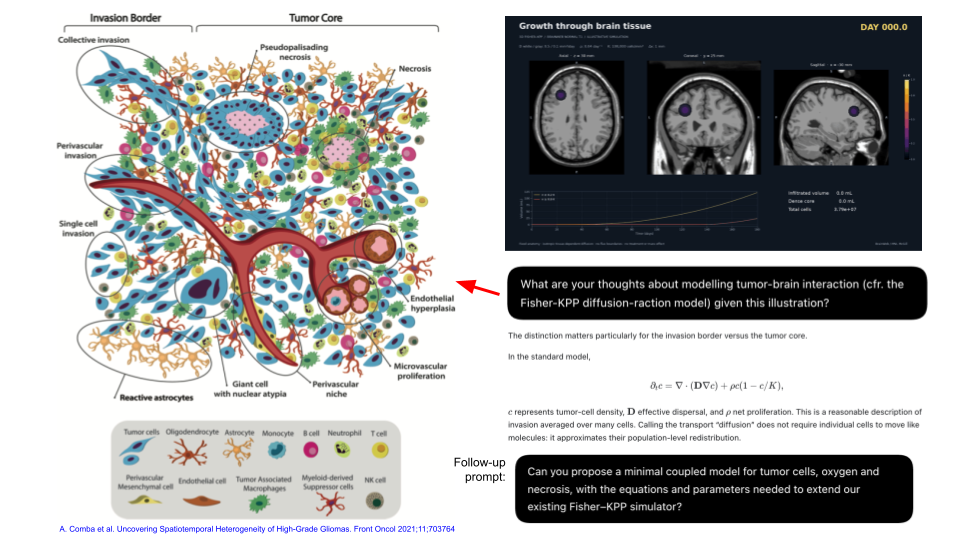
\includegraphics[width=.64\linewidth]{figures/talk/slide-19.png}}
\biopath
The histological schematic contrasts an invasion border with a heterogeneous tumour core. It depicts vessels, immune and stromal components, necrosis and different invasion patterns. Its role is to show how much biology is compressed when a model uses a single density field. The follow-up prompt asks for a minimal extension involving viable tumour, oxygen and necrotic material. That is a modelling proposal inspired by the diagram, rather than a derivation uniquely determined by it.

To interpret the proposal, tell a causal story in plain language. Oxygen can be supplied and consumed; low availability can affect survival; dead tissue can accumulate or be removed. Then ask which parts of that story the chosen equations actually represent and which remain assumptions. A dark region in an oxygen panel is a model state, not automatically a measured hypoxic region or an MRI compartment. The same caution applies to simulated necrotic material. Compare the extended model with the simpler Fisher--KPP reference under matched starting conditions. If the patterns differ, identify which added relationship caused the difference. A richer diagram can motivate a richer model, but additional biological vocabulary increases the need for clear definitions and discriminating observations.
\comppath
Begin with a state vector such as viable density, oxygen availability and necrotic material. Define the units and domain of each component before proposing coupling terms. Oxygen consumption should appear in its own balance; conversion from viable to necrotic material needs compatible units and signs. A production term for one compartment may require a corresponding loss from another, depending on the stated conservation assumptions. Normalised oxygen availability is not a concentration unless a scale has been defined.

The external implementation linked in the presentation guide supplies one illustrative closure: specific mathematical choices that complete the biological sketch. Those choices are unvalidated assumptions, not a unique model implied by the image. Test non-negativity, boundary behaviour and limiting cases, including whether disabling the added effects recovers the intended simpler dynamics. Identify parameters that the available observations could not determine separately. Increasing the number of adjustable coefficients can improve fit while making the mechanism less identifiable. For an exercise, propose two different oxygen-consumption rules that produce similar tumour outlines. Name an additional measurement that might distinguish them. The exercise shows why agreement with a single visible boundary offers limited evidence about the hidden processes represented in a coupled model.
\end{slidenotes}

\begin{slidenotes}{20}{Compare states with matched displays}{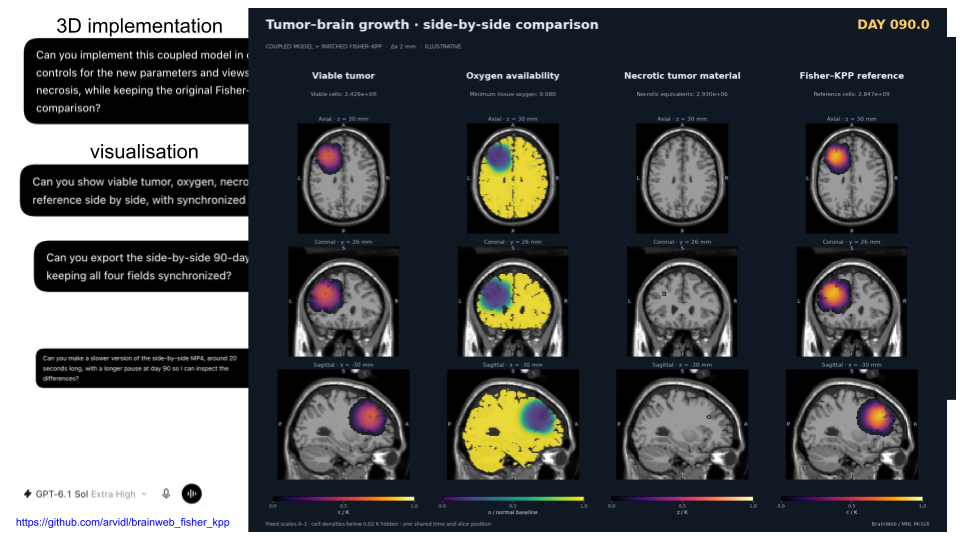
\includegraphics[width=.64\linewidth]{figures/talk/slide-20.png}}
\biopath
The four columns show simulated viable tumour, oxygen availability, necrotic material and a Fisher--KPP reference at a matched time and slice position. The comparison is useful because it separates quantities that a single coloured overlay could conflate. Read the colour bars before interpreting the images. A density fraction and normalised oxygen availability may both range from zero to one while referring to different states. A similar colour therefore does not imply a similar biological amount.

The anatomical background supports spatial orientation, while the overlays show outputs of an illustrative simulation. The extra oxygen and necrosis components have not thereby become measured patient properties. For a fair visual comparison, keep time, physical plane, colour scale and threshold conventions fixed. An apparent difference can otherwise be created by a changed display. Look for both local effects and changes in an integrated quantity. In particular, a thresholded volume asks how much tissue lies above a chosen value; integrated density asks how much modelled burden is distributed over the domain. Explain a case in which those quantities move differently. This develops the ability to read a simulation figure critically rather than equating a visually plausible animation with evidence that its mechanisms describe disease.
\comppath
Synchronisation is an experimental constraint. Store a common time index and physical slice coordinates for all fields, and compare the coupled model with a reference using documented initial conditions, grid and parameters. Fixed colour limits make changes over time interpretable; autoscaling can make a weak field look as intense as a strong one. State any masking or transparency threshold, because hidden low-density values still contribute to some numerical summaries.

For the local three-dimensional lesson, integrated density fraction is $B=v\sum_i u_i/1000$ in mL when each voxel has volume $v$ in mm$^3$. A thresholded volume is $V_\tau=v\sum_i\mathbf{1}[u_i\geq\tau]/1000$. The former is a volume-weighted model burden, and the latter is the volume of a thresholded set. Neither is an absolute cell count without the carrying-capacity scale. These definitions should accompany a numerical comparison even when the video supplies its own labels. Validate the renderer by checking that a stored voxel value agrees with its plotted position and colour. Validate the solver separately through numerical checks. The side-by-side view tests the consequences of modelling choices; it does not by itself establish which choice is biologically correct.
\end{slidenotes}

\begin{slidenotes}{21}{Agents produce different kinds of evidence}{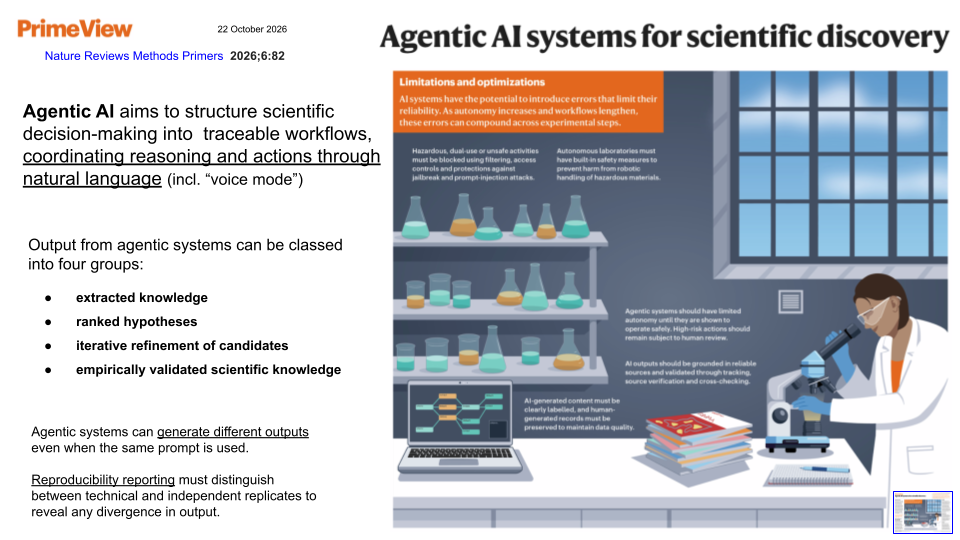
\includegraphics[width=.64\linewidth]{figures/talk/slide-21.png}}
\biopath
The PrimeView introduces agentic systems as workflows that coordinate reasoning and actions \citep{primeview2026}. The four output categories on the slide form a useful evidence ladder. Extracted information can support a literature map. Ranked hypotheses can guide a study. Iteratively refined candidates can focus resources. Empirically validated knowledge requires observations that test a claim. Producing an articulate hypothesis or an improved candidate does not skip those evidential steps.

Imagine an agent suggesting that an oxygen-sensitive growth model explains an imaging pattern. First check whether the cited studies support the extracted statements. Next examine whether the proposed hypothesis is distinguishable from alternatives. Then decide which observation could test it and whether the study design measures that observation adequately. A fluent chain connecting these stages can conceal a weak link. Natural-language or voice interaction can make the workflow easier to use, but the interface does not supply validation. Preserve the sources, intermediate decisions and failed tests that allow another investigator to examine the chain. The practical learning goal is to classify an output correctly and identify the next justified step. This makes AI assistance valuable without confusing the production of research material with the establishment of a scientific result.
\comppath
An agentic workflow can include a language model, tools, memory, branching logic and stopping criteria. The unit to reproduce is the resulting procedure, including tool versions and permissions, rather than a prompt alone. Save inputs, retrieved sources, tool arguments, outputs and decisions in a trace. A later reader should be able to identify where a claim entered the workflow and whether it was checked against an external observation.

Repeated runs under the same setup probe stochastic variability or technical repeatability. They are not independent biological replicates. Distinguish a rerun on the same data, a new sample from the same study and an independent study with its own acquisition and analysis. Those repetitions address different uncertainties. Also report unsuccessful runs where they affect the claimed reliability; selecting the best of many trajectories changes the meaning of the result. For an exercise, design an agent that proposes growth parameters from generated observations. Specify which actions it may take, which data it may inspect and when it must stop. Keep a forecast time point unavailable during fitting. The ability to inspect a complete trace then supports an audit of both procedural correctness and whether the final evaluation remained independent.
\end{slidenotes}

\begin{slidenotes}{22}{Place assistance inside the research design}{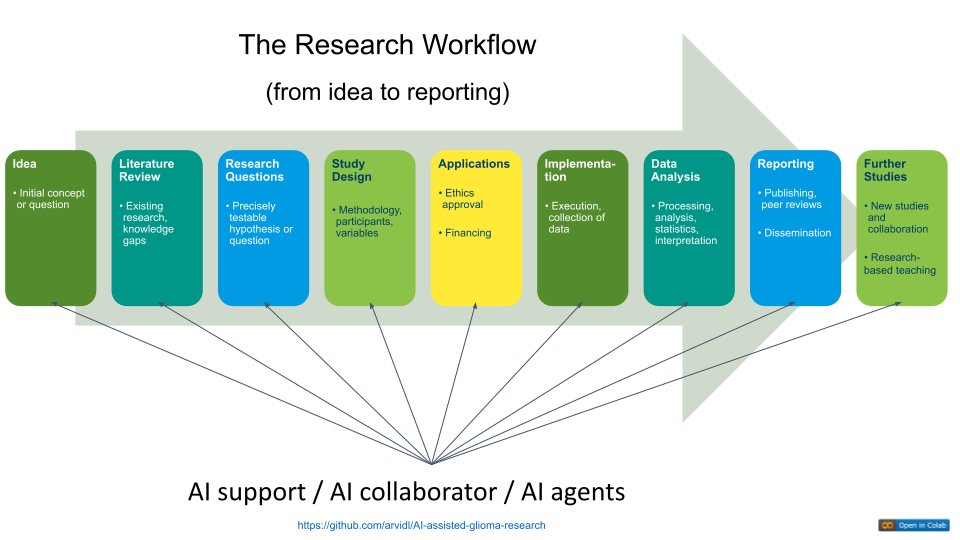
\includegraphics[width=.64\linewidth]{figures/talk/slide-22.png}}
\biopath
The workflow runs from an idea through literature review, a precise question, design, approvals and funding, implementation, analysis, reporting and further studies. AI support can enter at each stage, but each stage has its own criterion for success. A plausible research question must become answerable; an analysis must match the design; a report must preserve what was actually done. Ethics approval and appropriate data access belong to the study's conduct and cannot be inferred from a working analysis script.

Follow one example through the boxes: can serial imaging constrain a tumour-growth model sufficiently to forecast a later observation? Define which imaging quantity is measured, how examinations are aligned, and which time point is withheld. Decide what forecast error would matter before inspecting the final observation. Consider alternatives such as persistence of the most recent measurement. A model can fit earlier images closely without forecasting well, and a successful forecast does not establish a treatment effect. Use AI to draft plans, inspect code or organise evidence, while assigning scientific decisions to identifiable investigators. The diagram's return to research-based teaching closes the loop: explain the assumptions and failures, not only the result that survived to the final figure.
\comppath
The workflow can be represented as dependencies among research artefacts: a question, protocol, dataset version, analysis code, results and report. Record those dependencies so that changing an input identifies which outputs need to be recomputed. Freeze the primary evaluation before looking at its results. Automating a pipeline is useful, but a faithfully automated analysis can still answer an inappropriate question or use leaked information.

\coursenotebook{14c_growth_parameter_recovery.ipynb}{Notebook 14c} makes this distinction concrete with generated observations. It fits a diffusion scale and proliferation rate using selected earlier times, while day 90 remains withheld. The generating model, observation operator and parameter grid are controlled; the true pair is included among the candidates. This demonstrates parameter recovery and a forecast under favourable, specified conditions. It does not establish patient-level identifiability or clinical forecasting accuracy. The reference and fitting calculations use different time steps, but share the model family and spatial grid, so the test does not probe every form of model discrepancy. Compare the withheld forecast with persistence and explain both errors. Then propose one mismatch---an uncertain seed, changed observation operator or altered tissue map---that would make the task more realistic. State what additional evidence would be needed to interpret that new experiment.
\end{slidenotes}

\begin{slidenotes}{23}{A creative workflow and its provenance}{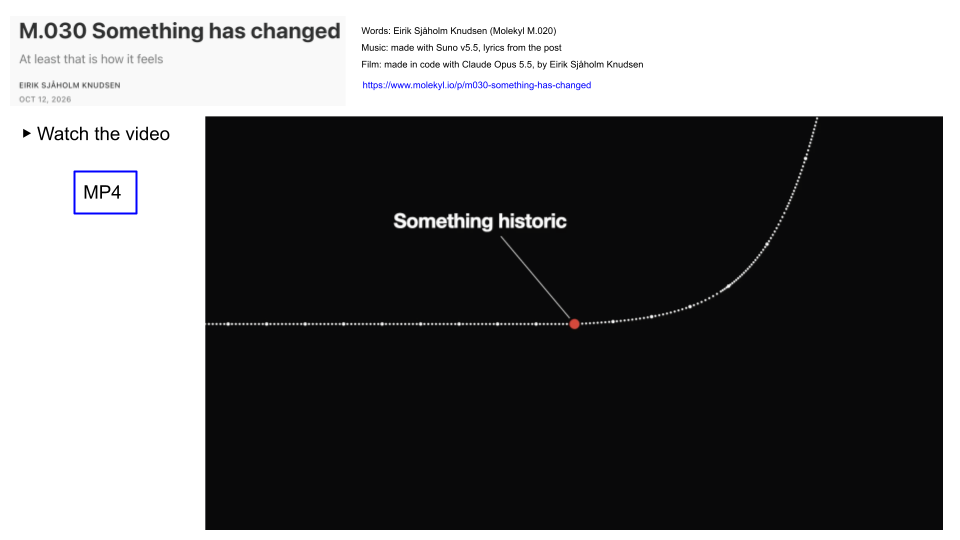
\includegraphics[width=.64\linewidth]{figures/talk/slide-23.png}}
\biopath
The slide introduces Eirik Sj\aa holm Knudsen's \emph{Something has changed}, a creative example combining human-written words, generated music and a film produced through code-assisted iteration. His accompanying post describes revisiting earlier writing in different media \citep{knudsen2026changed}. Use the example to examine collaboration and reception. A work can affect an audience through its words, rhythm, images and context even when parts of its production are automated. That response is evidence about the audience's encounter with the work, not a direct test of experience in the generating system.

The biomedical connection is communication. An animation or carefully chosen metaphor can make a difficult idea accessible, but emotional force can also make uncertain claims feel more settled than they are. If you use generated media to explain a model, distinguish the explanatory image from observed anatomy and state what the illustration simplifies. Ask viewers what they understood rather than assuming that attention implies understanding. In a short exercise, describe one concept twice: first as a factual paragraph, then as a proposed visual sequence. Identify which details the visual version leaves out and whether those omissions change the scientific meaning. The creative opportunity and the responsibility to preserve meaning belong together.
\comppath
Separate the stages of the media pipeline: source text, musical generation, visual specification, code, rendering and editing. Each has inputs and revision decisions. The model and tool names credited on the slide describe the reported production workflow; they do not provide a controlled comparison of those tools. Keep source material and generated artefacts distinguishable so that a later reader can identify which claims or creative decisions came from which stage.

For reproducibility, save the code and assets needed to render a chosen version, together with relevant settings and dependencies. Exact replay of a generation service may be unavailable even when deterministic rendering from saved assets is possible. These are different limits and should be documented separately. Evaluate a scientific animation by checking its correspondence to the underlying data or explanation, not only its visual quality. If the work suggests a dramatic reduction in labour, treat an AI-produced estimate of hypothetical human production time as an unvalidated estimate rather than a measured productivity study. Design a comparison with defined outputs and recorded effort if that claim matters. The example is strongest as an inspectable case of iterative creative collaboration, from which testable questions about quality, accessibility and effort can be developed.
\end{slidenotes}

\begin{slidenotes}{24}{Video interlude: observation and interpretation}{
\includegraphics[width=.64\linewidth]{figures/talk/slide-24.png}}
\biopath
The supplied static export contains a black panel with a red cross and a small credit to Knudsen and Molekyl. It does not contain a readable video frame. Treat this page as a companion to the preceding media example; motion, sound and additional content cannot be recovered from this PNG. The \href{https://www.molekyl.io/p/m030-something-has-changed}{creator's accompanying post} provides context for viewing the work separately. This distinction matters when an appendix must remain usable without the live presentation.

Use the interlude for a structured discussion. First describe something you actually observed in the work or its documented production. Next state your interpretation. Finally identify a claim that would require further evidence. For example, feeling that a sequence is compelling differs from establishing that it improves scientific understanding. If you have not watched it, keep the discussion about the documented workflow and avoid inventing its effects. In biomedical communication, the same discipline helps when a missing sequence, unavailable scan or incomplete record invites a plausible story. State the missing evidence, preserve what is known and specify what you would need to examine next. This is an exercise in careful interpretation as much as a discussion of creative technology.
\comppath
A presentation file, a static slide export and a rendered video preserve different information. A PNG can document layout and embedded credits while losing playback, timing, transitions or linked assets. The placeholder on this page illustrates what can be lost in a static export. It is not evidence that the original media lacked content or that a viewer saw the same panel during playback. Distinguish the source object from the particular export you can inspect.

For a computational exercise, specify a media manifest with the slide number, source asset, rendering method, duration where known, and a text alternative. Check that assets resolve and that the text alternative preserves the instructional purpose. If a video visualises simulated data, record the state files, time sampling, physical coordinates and colour mapping used to generate it. A static appendix can then link to the motion while retaining an explanation that stands alone. Evaluate accessibility and scientific faithfulness independently of whether playback succeeds. Apply the same principle to notebook outputs: a saved figure is evidence of a rendered result, whereas rerunning the computation additionally tests whether the documented environment and inputs reproduce it. The missing frame becomes a useful lesson in what a reproducible artefact must preserve.
\end{slidenotes}

\begin{slidenotes}{25}{Synthesis and a next experiment}{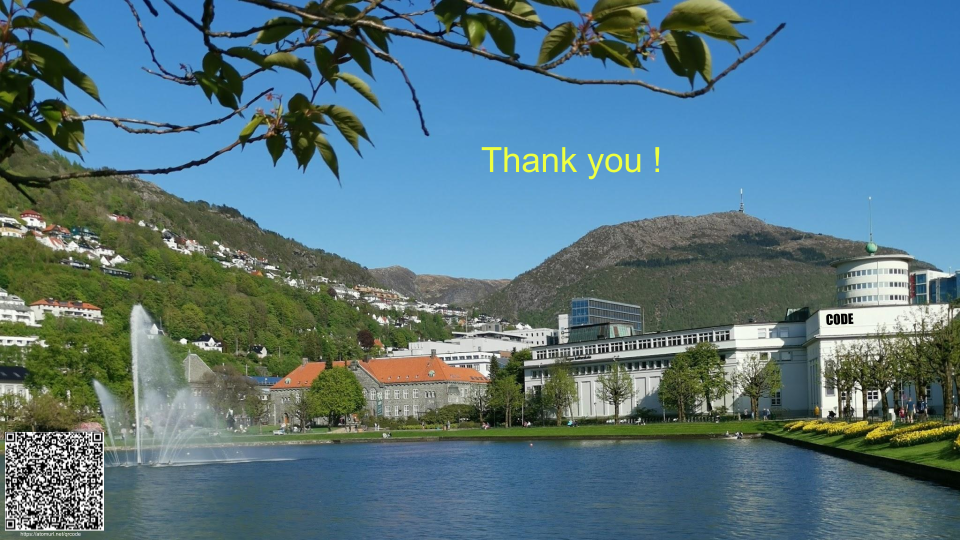
\includegraphics[width=.64\linewidth]{figures/talk/slide-25.png}}
\biopath
The closing image is an invitation to return from the presentation to a question in your own work. Select one model claim and explain it using the distinctions developed across the slides. What was measured? What was represented? Which process was assumed? What would a person do with the result? A useful synthesis connects these questions rather than concluding that machines are either wholly equivalent to people or irrelevant to human understanding.

For a concrete final exercise, interpret a positive test before recommending an action. With 1\% prevalence and both sensitivity and specificity at 90\%, a hypothetical group of 10,000 contains 90 true positives and 990 false positives. Thus only about 8.3\% of positive results are true positives. This expected-count example is constructed, not a measured diagnostic study. The appropriate action also depends on consequences and further evidence. \coursenotebook{15_ppv_and_decisions.ipynb}{Notebook 15} develops the calculation. Explain it to a colleague without beginning with a formula, and ask the colleague to describe the result back to you. Finish by naming one observation that would change your conclusion. That final sentence turns a confident-looking answer into a claim whose limits another person can examine.
\comppath
Choose a small reproducible investigation and state its purpose, algorithm and implementation. The course offers several routes: an input intervention in segmentation, a numerical limiting case, a threshold-versus-density comparison or a withheld growth forecast. Specify which output would count against your preferred explanation. Preserve the input, parameters, code version and result so that the test can be repeated. Report a failure with enough detail to make it useful for the next attempt.

For a final decision exercise, suppose $p$ is a calibrated event probability, a false positive costs one unit and a false negative costs four, with zero cost assigned to correct decisions. Acting has expected loss $1-p$; not acting has loss $4p$. Acting is favoured when $p>0.2$, with a tie at the boundary. These stipulated losses illustrate a decision rule; they are not clinical recommendations. Distinguish this probability threshold from an operating threshold used to obtain a classifier's sensitivity and specificity. The calculation links prediction to action only through its explicit assumptions. End your investigation with the same discipline: state the measured result, the assumptions needed for its interpretation, and the additional test required before extending the claim to a new population, mechanism or use.
\end{slidenotes}
\endgroup
